% \Huge

\section{Information loss and potential recovery}

We studied information loss due to gravitational collapse. Our two main observational probes (CMB and Galaxy surveys) are widely separated by an era from which we have very little information, and which contains such important events as the formation of the first stars and galaxies. It is, therefore, in our interest to find ways of using the data we collect about our Universe today to recover information about the past. Reconstruction techniques have been widely used to recover information on the Baryon Acoustic Peak, but here we look to even smaller scales. Our aim was to test the limits of reconstruction as well as to look at more realistic methods and test their performance.

In Chapter 2, we proved that some information will never be recovered. To show this, a perfect reconstruction was performed. We measured the density field at the particle positions and used the knowledge of the initial particle positions to reconstruct it. Because we do not (and cannot) measure the density field in an infinity of locations we cannot capture all of its information. This means, no reconstruction is capable of perfectly recovering the primordial density field.

Figure~\ref{fig:3.2} shows the normalized cross spectra of our reconstructed fields with the initial density field (versus the original correlation). Our reconstruction recovers plenty of  intermediate scale information and the two stay correlated to very small scales. However, on these very small scales, they do decorrelate. This information can never be recovered by reconstructing the density field. The plot shows the most amount of information that could ever be recovered from each redshift. In a way, it shows the limit of what we can ever hope to learn about the primordial density field. 

We have also shown that two of the limiting factors in reconstruction are the resolution used and the redshift. Both of these can be improved upon in practice. More and more information is destroyed with the progress of time. By detecting matter further back in time, we increase the amount of information we can recover. On the resolution side, our limitations are the size of galaxies and how many of them we can detect in a certain volume. Galaxies are also biased tracers of matter, therefore galaxy surveys might not be our best option. A very promising future probe is the Square Kilometre Array (SKA),\todo{ref} as it will push both boundaries at the same time. Its goal is to detect atomic hydrogen before reionisation (using the 21cm emission). As we are looking much further back in time ($z>10$) and directly at the matter distribution, this probe will lead to incredible advancements in our knowledge of the early Universe.


After studying the limits of reconstruction, we turned our attention to more realistic methods in Chapter 3. In particular, we looked at reconstruction methods within the Lagrangian framework. We first start by performing a Zel'dovich reconstruction. Particle velocities are used to calculate a displacement field within the first order approximation of Lagrangian Perturbation Theory (the Zel'dovich Approximation). As before, we calculated the density field at the particle positions and then applied the displacement field to move them back in time. The density field is also carried back in time and reconstructed. We showed that the method works very well when starting at high redshifts ($z=9$). However, when starting at low redshifts, this method creates an anti-correlation on the largest scales. This is probably caused by the fact that at those redshifts ($z=0$) most particles have highly non linear velocities, however this phenomenon is not well understood. We left this Zel'dovich reconstruction as just an intermediate step, because of its lack of realism (in practice we could not measure so many velocities so accurately) and its poor performance at low redshifts.

In order to improve the realism and low redshift performance of the method we investigated ways of smoothing the velocity field. We present two methods for achieving this. For the first one, we just average velocities over 1 Mpc and 10 Mpc scales respectively, and interpolate the velocities back at the particle positions. For the second one, we average velocities over smaller scales (0.5 Mpc) and apply a Gaussian filter to smooth this average velocity field over 1 Mpc and 10 Mpc scales respectively. After that, we again interpolate the velocities back at the particle positions. Finally, in both cases we use the smoothed velocities and the Zel'dovich approximation to move the particles (and the density field with them) back in time. These methods are more realistic because we are giving up the accurate and precise knowledge of all the particle velocities. Instead, we now have an average velocity field over certain scales, and this could be measured in practice. 

Figure~\ref{fig:4.2} shows the impact of smoothing velocities on information recovery. When we smooth the velocity field, we are giving up some information and this can be seen in a small loss of correlation on intermediate scales. When comparing the two smoothing methods, we found that normal averaging of particle velocities across the scales of interest (1 Mpc and 10 Mpc) does not lead to a large improvement in the $z=0$ correlation (compared to the the previous Zel'dovich reconstruction). In fact, using this method, the largest scales achieve almost perfect anti-correlation. This is a very interesting result that should be studied further. On the other hand, the second method of using smaller bins to average velocities and then applying a Gaussian filter, works much better. In this case we recover intermediate scale information very well, and the largest scales do not become anti-correlated. Therefore, based on these results, we recommend smoothing the velocity field using small bins (0.5 Mpc) to average velocities and applying a Gaussian filter to smooth velocities over the scales of interest.

The best reconstruction we achieved with this method was using Simulation B (Figure~\ref{fig:4.5}). In that case, our reconstructions perform better than the original on almost every scale. However, the amount of intermediate scale information recovered is very small. The decorrelation scale does decrease, but very little compared to the perfect reconstruction. On the other hand, when applying the same method to Simulation A (Figure~\ref{fig:4.6}), we obtain better intermediate scale correlation, but the large scales start to decorrelate. This information trade-off is a trend we have seen throughout Chapter 3. Within the Zel'dovich approximation, whenever we use more velocity information, we recover more intermediate scale information. On the other hand, we lose the large scale correlation that was there to begin with. In the most extreme cases (Figure~\ref{fig:last}), we obtain almost perfect anti-correlation of the largest scales. However, we do succeed in our objective of pushing the boundaries of reconstruction to scales smaller than the BAO. 


\begin{figure}
    \centering
    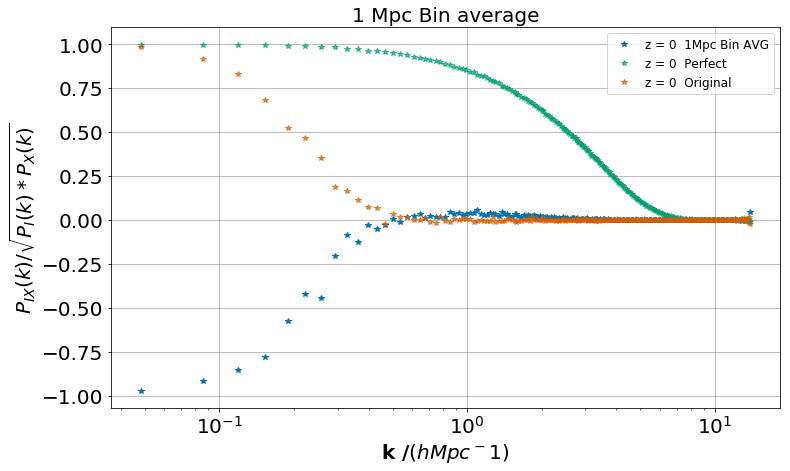
\includegraphics[width=1\columnwidth]{images/realRecon/1MpcBinAvg.png}%
    
    \caption{
        Simulation A reconstruction
        }
        
        \label{fig:last}
\end{figure}

\section{Future Work}
    
There were many interesting results discovered during this project. Perhaps the best example is the almost perfect anti-correlation obtained in some cases. Figure~\ref{fig:last} shows one of the most extreme cases. To perform this reconstruction, we averaged velocities over 1 Mpc bins, interpolated the velocities back onto the particles and then applied the Zel'dovich offset as described in Chapter 3. The resulting correlation is almost a (negative) mirror image of the original correlation. We saw in Section 3.1.3 that the Zel'dovich reconstruction leads to some anti-correlation on the largest scales when starting at low redshifts. This could be explained by the fact that most particles are past shell crossing at this stage. Also, high density collapsed regions tend to have higher peculiar velocities. Because we just use these velocities once to calculate the displacement (we don't re-evaluate it as we go back in time) we are displacing most of the matter in these regions. However, we know that this must have been a large overdensity at early times (in order to have formed a massive filament). This then leaves us with an anti-correlation. On the other hand, a perfect anti-correlation of the largest scales is very hard to explain and should be studied further. 

Another possible extension of this work would be to smooth the density field. When performing the reconstruction we have assumed perfect knowledge of the final density field, which of course is not the case in practice. A further step that would increase the realism of this method would be to also smooth the density field in a manner similar to our smoothing of the velocity field.

The perfect reconstruction has achieved vastly better results than any realistic reconstruction we have attempted. This leads us to conclude that there is much space for the improvement of these methods. We have only used the first order approximation to Lagrangian Perturbation Theory. Higher order approximations could perform better, and also solve some of the problems we encountered.
    
